\documentclass[border=0.5cm]{standalone}
\usepackage{color}
\usepackage{tikz}
\usetikzlibrary{shapes,arrows,arrows.meta,fit,positioning}

\newcommand{\defaultwidth}{5cm}
\tikzset{
    auto, node distance = 2cm,
    stage/.style = { draw, thick, rectangle, align=center,
        text width = \defaultwidth, 
        font=\bfseries,
        rounded corners=2mm, 
        minimum width = \defaultwidth
    },
    note/.style = { draw, very thin, rectangle, dashed, align=center,
        node distance = 0.5cm,
        text width = \defaultwidth - 1cm, 
        font=\footnotesize,
        minimum width = \defaultwidth - 1cm
    },
    arrow/.style = { ->, very thick },
    arrow_text/.style = { align=center,
        pos = 0.5,
        text width = 3cm, 
        font = \scriptsize
    }
}

\begin{document}
    \begin{tikzpicture}
        \node[stage] (0) at (0,0)
            {Set of points \\ 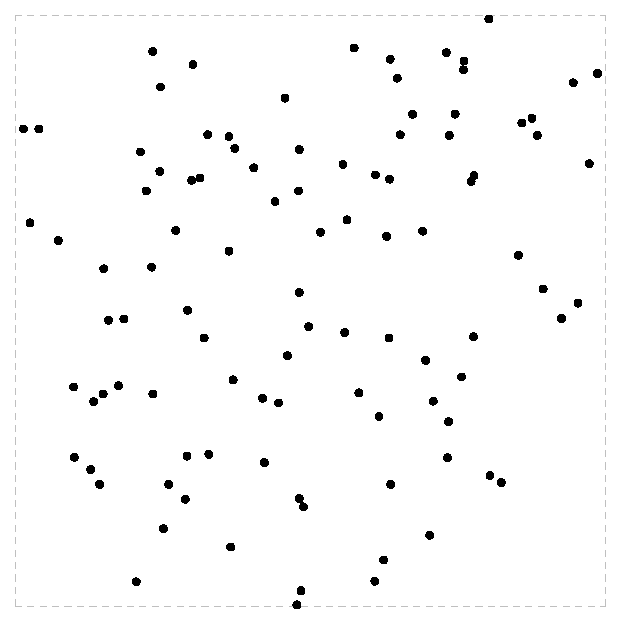
\includegraphics[width=\defaultwidth]{MF_stages/points}};
        \node[stage] (1) [right = of 0]
            {Partitioning points \\ 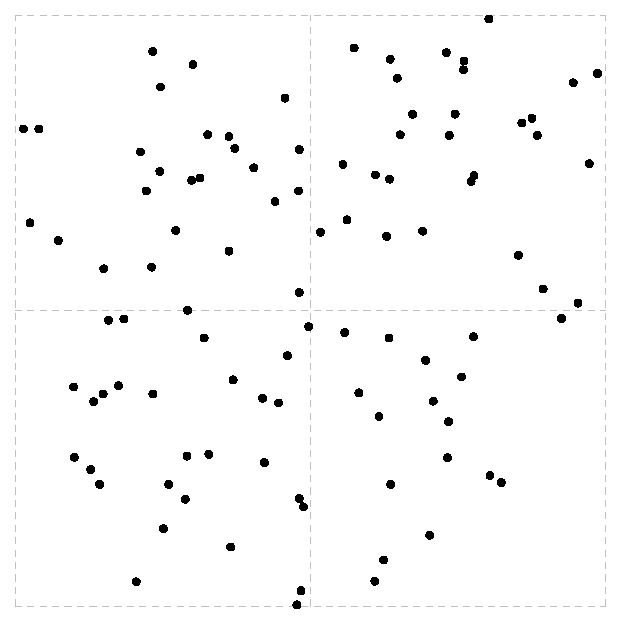
\includegraphics[width=\defaultwidth]{MF_stages/partitions_points}};
        \node[stage] (2) [right = of 1]
            {Finding pairs \\ 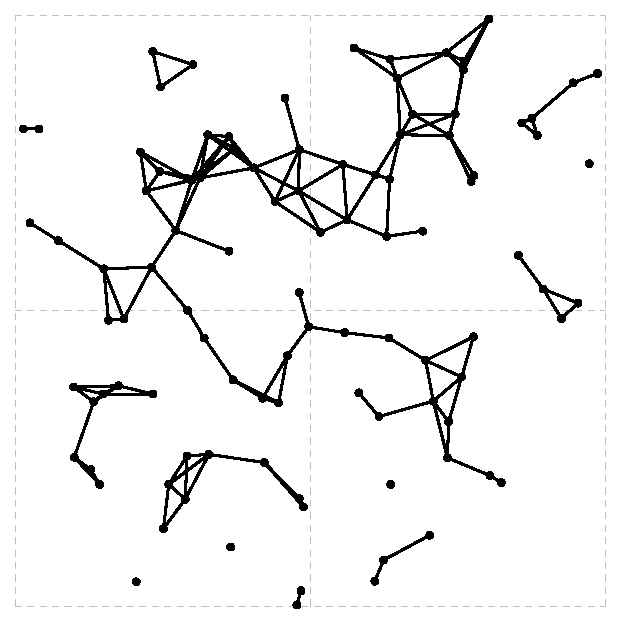
\includegraphics[width=\defaultwidth]{MF_stages/pairs}};
        \node[stage] (3) [right = of 2] 
            {Computing centers \\ 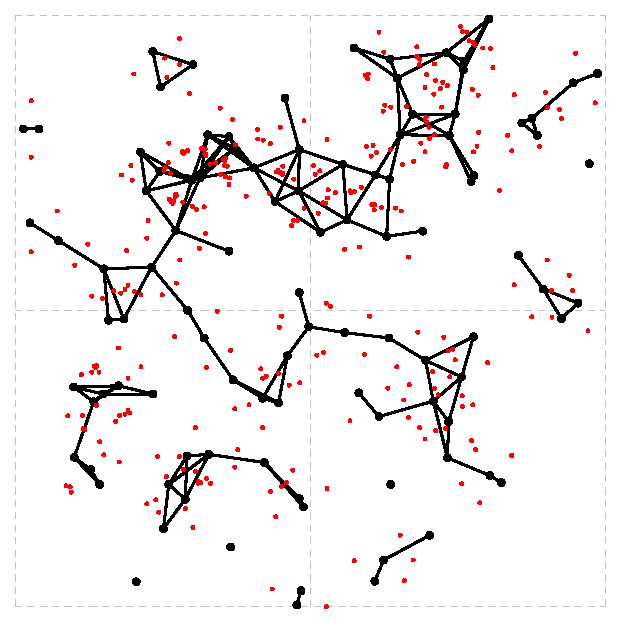
\includegraphics[width=\defaultwidth]{MF_stages/centers}};
        \node[stage] (4) [right = of 3] 
            {Finding disks \\ 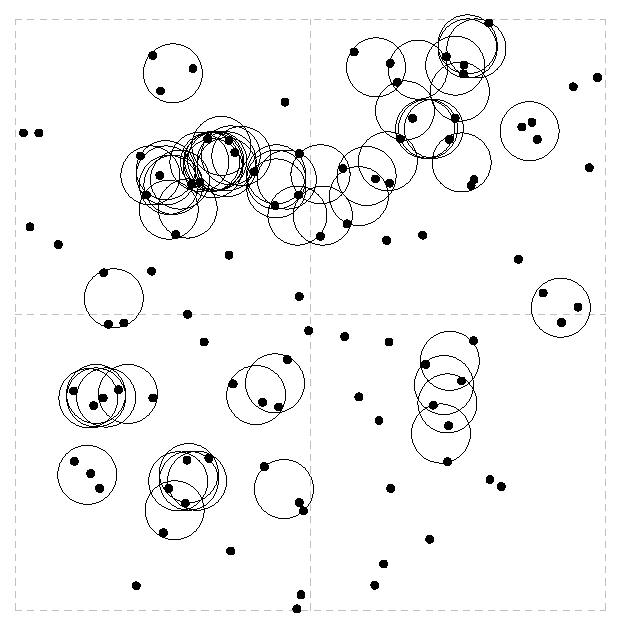
\includegraphics[width=\defaultwidth]{MF_stages/disks}};
        \node[stage] (5) [right = of 4] 
            {Partitioning disks \\ 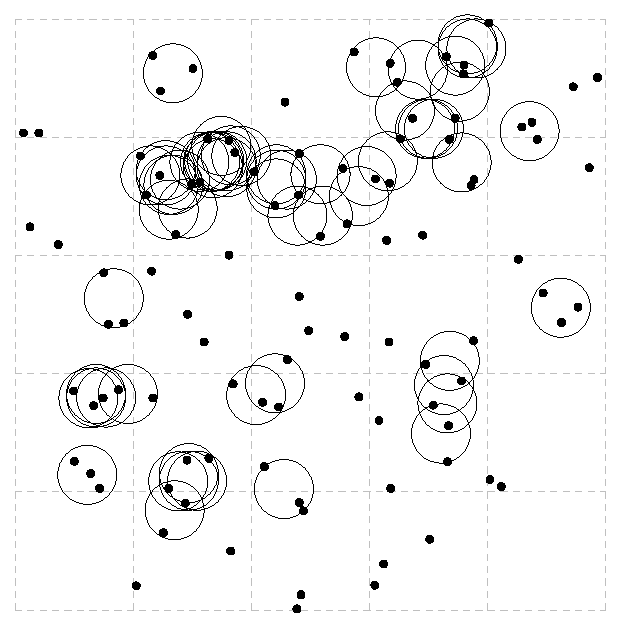
\includegraphics[width=\defaultwidth]{MF_stages/partitions_disks}};
        \node[stage] (6) [right = of 5] 
            {Maximal disks \\ 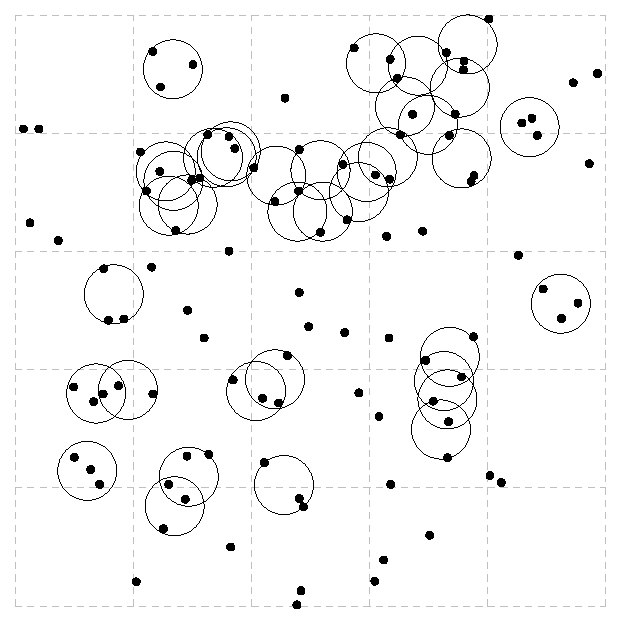
\includegraphics[width=\defaultwidth]{MF_stages/maximals}};

        \node[note] (11) [below = of 1] {Coarse grid used\\ for spatial join operation};            
        \node[note] (21) [below = of 2] {Points at less than $\varepsilon$ distance form a pair};            
        \node[note] (31) [below = of 3] {Two centers from each pair are computed};            
        \node[note] (41) [below = of 4] {Disks with less that $\mu$ points are removed};            
        \node[note] (51) [below = of 5] {Fine grid used\\ for LCM prunning};            
                        
        \draw[arrow] (0) -- node[arrow_text]{Point \\ dataset} (1);
        \draw[arrow] (1) -- node[arrow_text]{Point \\ dataset} (2);
        \draw[arrow] (2) -- node[arrow_text]{Pair \\ dataset} (3);
        \draw[arrow] (3) -- node[arrow_text]{Center \\ dataset} (4);
        \draw[arrow] (4) -- node[arrow_text]{Disk \\ dataset} (5);
        \draw[arrow] (5) -- node[arrow_text]{Disk \\ dataset} (6);
        
    \end{tikzpicture}
\end{document}
